\section{Wave Variables Resilience to Time Varying Delays}
\label{S:wave_vars_time_delay}
It is well established for the continuous-time plant and controller framework that wave variables allow both {\it effort} and {\it flow} variables to be transmitted over a network in a \passive\ manner when subject to arbitrary fixed time delays and data dropouts \cite{anderson92:_asymp_stabil_for_force_reflec, niemeyer04:_telem}.
More recently the conditions required on the time-delay characteristics of discrete-time wave variables has been established.  From some of the work involving discrete-time wave variables the engineer may be led to believed that any arbitrary discrete-time delay can be tolerated.  This indeed is not the case, Proposition~\ref{P:passive_t_d_con} makes this explicitly clear by summarizing recent observations  made in \cite{cst08, stramigioli05:_sampl_hamil, kottenstette07:_stabl_digit_contr_networ_contin, kottenstette08:_wirel_digit_contr_of_contin}.
\begin{figure}
  \centering
  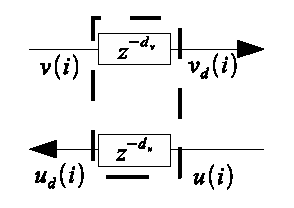
\includegraphics[width=1.8in]{figures/prop_delays}
  \caption{Generalized wave variable delay figure.}
  \label{fig:prop_delays}
\end{figure}
\begin{proposition}
\label{P:passive_t_d_con}
More generally, given the two pairs of wave variables $(u(i),v_d(i))$, $(u_d(i),v(i))$ depicted in Fig.~\ref{fig:prop_delays} in which the received-waves with the $d$-subscript are related to their corresponding non-delayed transmitted-counterparts such that
\begin{align*}
u_d(i) = \begin{cases}
u(i-d_u(i)),\ \text{if $d_u(i) \leq i$}\\
0,\ \text{otherwise.}
\end{cases}\\
v_d(i) = \begin{cases}
v(i-d_v(i)),\ \text{if $d_v(i) \leq i$}\\
0,\ \text{otherwise.}
\end{cases}
\end{align*}
where $d_u(i),\ d_v(i) \in \{1,2,\dots,\}$ is the respective delay at time $i$.  A necessary condition for 
\begin{equation}
\label{E:key_wave_equation}
\sum_{i=0}^{N-1}u\tr (i)u(i) - v_d\tr (i) v_d(i) \geq \sum_{i=0}^{N-1} u_d\tr (i)u_d(i) - v\tr (i) v(i)
\end{equation}
or equivalently
\begin{equation*}
\sum_{i=0}^{N-1}u\tr (i)u(i) - u_d\tr (i) u_d(i) + \sum_{i=0}^{N-1} v\tr (i)v(i) - v_d\tr (i) v_d(i) \geq 0
\end{equation*}
to be satisfied for all $N > 0$ is that both
\begin{align*}
\sum_{i=0}^{N-1}u\tr (i)u(i) - u\tr (i-d_u(i)) u(i-d_u(i)) \geq& 0\ \text{and}\\
\sum_{i=0}^{N-1} v\tr (i)v(i) - v\tr (i-d_v(i)) v(i-d_v(i)) \geq& 0
\end{align*}
are satisfied for all $N > 0$.  Therefore:
\begin{enumerate}[I.]
\item \label{P:p_t_d_c_1}if delays are fixed ($d_u(i)=d_u, d_v(i)=d_v$) then \eqn{E:key_wave_equation} is always satisfied,
\item \label{P:p_t_d_c_2}if the delays are such that data is always dropped ($d_u(i)=d_v(i)=(i+1)$) then \eqn{E:key_wave_equation} is always satisfied,
\item \label{P:p_t_d_c_3}if the delays are switched arbitrarily between a constant delay or a drop-out delay ($d_u(i)\ \in \{d_u,(i+1)\}$ and ($d_v(i)\ \in \{(i+1),d_v\}$)) then \eqn{E:key_wave_equation} is always satisfied,
\item \label{P:p_t_d_c_4}if the delays are such that no duplicate wave-transmissions are processed then \eqn{E:key_wave_equation} is always satisfied, more precisely if we denote the set of received indexes up to time $N-1$ for $u_d$ and $v_d$ as $\mathcal{D}_u = \{0-d_u(0),1-d_u(1),\dots,(N-1)-d_u(N-1)\}$ and $\mathcal{D}_v = \{0-d_v(0),1-d_v(1),\dots,(N-1)-d_v(N-1)\}$ respectively and
\begin{itemize}
\item each index $i \in \{0,1,\dots,N-1\}$ appears in $\mathcal{D}_u$ no more than once and
\item each index $i \in \{0,1,\dots,N-1\}$ appears in $\mathcal{D}_v$ no more than once.
\end{itemize}
An example of a delay which violates this final condition is when $d_u(i)=i$ in which $\mathcal{D}_u=\{0,0,\dots,0\}$ and the index $0$ appears $N$ times.
\end{enumerate}
\end{proposition}
 TCP/IP is a transmission protocol which will satisfy \eqn{E:key_wave_equation} however the UDP protocol could replicate packets and violate \eqn{E:key_wave_equation}.  Applications which choose to use UDP can be easily modified to satisfy Propositions~\ref{P:passive_t_d_con}-\ref{P:p_t_d_c_4}.
\subsection{Additional Proofs}
\subsubsection{Lemma~\ref{L:pj_ef_p_c_i}}
\label{S:pj_ef_p_c_i}
\begin{IEEEproof}
Summing the both sides of \eqn{E:passive_power_junction} with respect
to index $i \in\ \{0,1,\dots,N\}$ we have:
\begin{equation}
\label{E:pj_eq_1}
\begin{split}
\twonorm{(u_{\mathsf{n}})_N}^2-\twonorm{(v_{\mathsf{n}})_N}^2 \geq&
\sum_{\mathsf{j}=1}^{\mathsf{m}}(\twonorm{(u_{\mathsf{j}})_N}^2-\twonorm{(v_{\mathsf{j}})_N}^2)\\
& \quad + \sum_{\mathsf{j}=\mathsf{m} +1}^{\mathsf{m_c}}
(\twonorm{(u_{\mathsf{j}})_N}^2-\twonorm{(v_{\mathsf{j}})_N}^2), 
\end{split}
\end{equation}
take the left-hand-side (\LHS) of \eqn{E:ps_ph_cor} into the \LHS\ of
\eqn{E:pj_eq_1}, likewise substitute the right-hand-side (\RHS) of
\eqn{E:dig_con_uv_ef} into the \RHS\ of \eqn{E:pj_eq_1} which yields
\eqn{E:pj_ef_p_c_i}.
\end{IEEEproof}
\subsubsection{Theorem~\ref{T:main_theorem}}
\label{S:main_theorem}
\begin{IEEEproof}
We recall from Lemma~\ref{L:pj_ef_p_c_i} that if any of the conditions listed in
Proposition~\ref{P:passive_t_d_con} are met for the wave variable
communication time-delays $c_{\mathsf{j}}(i)=c_{\mathsf{n}}(i)=d_u(i)$, $p_{\mathsf{j}}(i)=p_{\mathsf{n}}(i)=d_v(i)$ that 
\begin{equation}
\label{E:main_assumption}
\innerprod{f_{{\mathsf{pn}}}}{e_{{\mathsf{dcn}}}}_{NT_s} \geq
\sum_{{\mathsf{j}}=1}^{{\mathsf{m_c}}} \innerprod{e_{\mathsf{cj}}}{f_{\mathsf{dpj}}}_N
\end{equation}
holds for all $N \geq 1$.
We recall, that the \sop\ plant satisfies
\begin{equation}
\label{E:sop_plant}
\innerprod{f_{\mathsf{pn}}}{e_{\mathsf{pn}}}_{NT_s} \geq \epsilon_{\mathsf{pn}} \twonorm{(f_{\mathsf{pn}})_{NT_s}}^2 - \beta_{\mathsf{pn}}
\end{equation}
while each \sop\ controller for ${\mathsf{j}} \in \{1,\dots,{\mathsf{m_c}}\}$ satisfies
\eqn{E:sop_controller}.
\begin{equation}
\label{E:sop_controller}
\innerprod{e_{\mathsf{cj}}}{f_{\mathsf{cj}}}_N \geq \epsilon_{\mathsf{cj}} \twonorm{(e_{\mathsf{cj}})_N}^2 - \beta_{\mathsf{cj}}
\end{equation}
In addition, we can substitute \eqn{E:ipesh_con_e2} into
\eqn{E:sop_controller} which yields
\begin{equation}
\label{E:sop_controller_nts}
\innerprod{e_{\mathsf{cj}}}{f_{\mathsf{cj}}}_N \geq \frac{\epsilon_{\mathsf{cj}}}{T_s
  k_s^2}\twonorm{(e_{\mathsf{cj}})_{NT_s}}^2 - \beta_{\mathsf{cj}}.
\end{equation}
Substituting, $e_{\mathsf{dcn}} = r_{\mathsf{pn}}-e_{\mathsf{pn}}$ and $f_{\mathsf{dpj}} = f_{\mathsf{cj}} -
r_{\mathsf{cj}}$ into \eqn{E:main_assumption} yields 
\begin{equation*}
\innerprod{f_{\mathsf{pn}}}{r_{\mathsf{pn}}-e_{\mathsf{pn}}}_{NT_s} \geq 
\sum_{\mathsf{j}=1}^{\mathsf{m_c}} \innerprod{e_{\mathsf{cj}}}{f_{\mathsf{cj}}-r_{\mathsf{cj}}}_N
\end{equation*}
which can be rewritten as
\begin{align}
\label{E:main_l2_inequality}
\innerprod{f_{\mathsf{pn}}}{r_{\mathsf{pn}}}_{NT_s} +
\sum_{\mathsf{j}=1}^{\mathsf{m_c}} \innerprod{e_{\mathsf{cj}}}{r_{\mathsf{cj}}}_N \geq \nonumber\\
\innerprod{f_{\mathsf{pn}}}{e_{\mathsf{pn}}}_{NT_s} + 
\sum_{\mathsf{j}=1}^{\mathsf{m_c}} \innerprod{e_{\mathsf{cj}}}{f_{\mathsf{cj}}}_N
\end{align}
so that we can then substitute \eqn{E:sop_plant}, 
\eqn{E:sop_controller_nts}, and \eqn{E:ipesh_con_ip} into \eqn{E:main_l2_inequality} to yield 
\begin{align}
\label{E:main_l2_inequality_final}
\innerprod{f_{\mathsf{pn}}}{r_{\mathsf{pn}}}_{NT_s} +
\sum_{\mathsf{j}=1}^{\mathsf{m_c}} \innerprod{e_{\mathsf{cj}}}{r_{\mathsf{cj}}}_{NT_s} \geq \nonumber\\ 
\epsilon[\twonorm{(f_{\mathsf{pn}})_{NT_s}}^2 + 
\sum_{\mathsf{j}=1}^{\mathsf{m_c}} \twonorm{(e_{\mathsf{cj}})_{NT_s}}^2] - \beta
\end{align}
in which $\epsilon = \min(\epsilon_{\mathsf{pn}},\frac{\epsilon_{\mathsf{cj}}}{T_s
  k_s^2}),\ \mathsf{j} \in \{1,\dots,\mathsf{m_c}\}$ and $\beta =
\beta_{\mathsf{pn}} + \sum_{\mathsf{j}=1}^{\mathsf{m_c}} \beta_{\mathsf{cj}}$.
Thus \eqn{E:main_l2_inequality_final} satisfies \cite[Definition~4-iii)]{kottenstette08:_contr_of_multip_networ_passiv}
for \sopy\ in which the input is the row vector of all controller and
plant inputs $[r_{\mathsf{c1}},\dots,$ $r_{\mathsf{cm_c}},r_{\mathsf{pn}}]$, and
the output is the row vector of all controller and plant outputs
$[e_{\mathsf{c1}},\dots,$ $e_{\mathsf{cm_c}},f_{\mathsf{pn}}]$.  When we let
$\epsilon_{\mathsf{pn}} = \epsilon_{\mathsf{cj}} = 0$ we see that all the plants and
controllers are \passive, therefore the system depicted in
Fig.~\ref{fig:resilient_control_net} is \passive.
\end{IEEEproof}